\subsubsection{Flöde vid transient förlopp}

%To regerenate the figures use /code/pdesolver/calculateRisetime.m
%with the argument /code/pdesolver/wallstep.mat

\begin{figure}[hpbt]
\centering

\subfloat[Energiflöde ut från insidan av en vägg med $0,5\mbox{m}$ tegel.]{
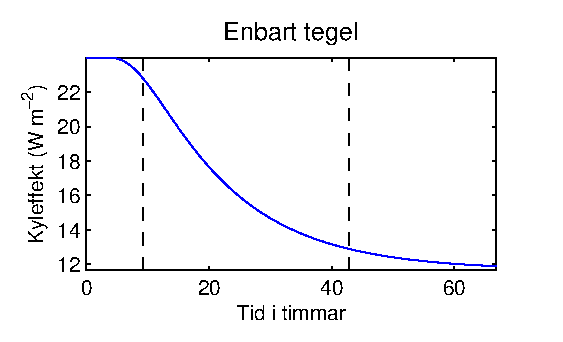
\includegraphics[width=6cm]{images/noinsulationstep.eps}
}\vspace{5mm}
\subfloat[Energiflöde ut från insidan av en vägg med $0,5\mbox{m}$ tegel och
$1\mbox{dm}$ tilläggsisolering bestående av mineralull.]{
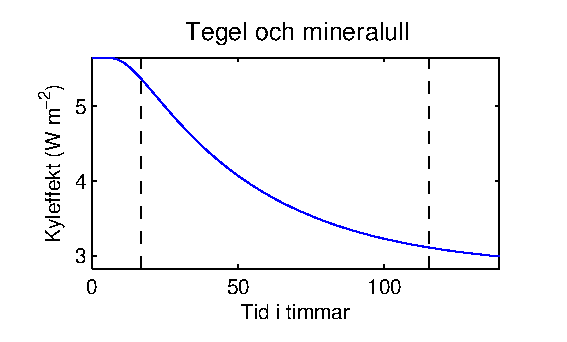
\includegraphics[width=6cm]{images/insulationstep.eps}
}
\caption{Energiflödet ut från insidan av en vägg där jämviktsläge med
$\unit[0]{^\circ C}$ på utsidan. Temperaturen förändras sedan
till $\unit[10]{^\circ C}$ vid tiden $t=0$. Insidan av väggen är satt till
konstanta $\unit[20]{^\circ C}$. De streckade linjerna markerar $\unit[10]{\%}$
fall samt $\unit[90]{\%}$ fall. Falltiden för dessa två väggar beräknades sedan
till $\unit[34,7704]{ timmar}$ för väggen utan isolering samt
$\unit[98,8372]{ timmar}$ för väggen med isolering. En annan intressant notering
är att det tog $\unit[9,5651]{ timmar}$ och $\unit[16,7533]{ timmar}$ för
energiflödet att falla $\unit[10]{\%}$. Beräkningarna är genomförda med finita
elementmetoden med $\unit[0,5]{m}$ tegel och $\unit[1]{dm}$ mineralull.}
\end{figure}
